
\documentclass[]{openjournal}

\bibliographystyle{apj}
\usepackage{graphicx}
\usepackage[suffix=]{epstopdf}
\usepackage[export]{adjustbox}
\usepackage{natbib}
\usepackage{amsmath}
\usepackage{url}
\usepackage{xspace}

%    Make Scientific Notation
\providecommand{\e}[1]{\ensuremath{\times 10^{#1}}}

% make the word Kepler italicized
\newcommand{\Kepler}{\textsl{Kepler}\xspace}


\begin{document}
%%%%%%%%%%%%%%%%%%%%%%
\title{}

\shorttitle{}
\shortauthors{Davenport et al.}

\author{
	James R. A. Davenport\altaffilmark{1,2,3}
	}

\altaffiltext{1}{Corresponding author: James.Davenport@wwu.edu}
\altaffiltext{2}{Department of Physics \& Astronomy, Western Washington University, Bellingham, WA 98225}
\altaffiltext{3}{NSF Astronomy and Astrophysics Postdoctoral Fellow}
 

%%%%%%%%%%%%%%%%%%%%%%%%%%%%%%
\begin{abstract}
The idea is simple: ET's would place artificial satellites in orbit around stars surrounding their home star system. The orbit period of the remote artificial satellites (or beacons) would be proportional to the distance from the remote star to the home star system. Each remote beacon system would be part of a network map leading to the home system. If the orbital period vs beacon distance relationship was known, the exact location of the home system could be triangulated using only a subset of the beacons.
\end{abstract}

%%%%%%%%%%%%%%%%%%%%%%%%%%%%%%
\section{Introduction}

Previous work has suggested looking for SETI signals from interstellar ``beacons''
\cite{benford2008}
However, most such work has been focused on using lasers or other means to out-shine a parent star, often observed using spectroscopy \cite{reines2002}. This is every expensive way to stand out, and a slow way to find it, and so far has no success in discovering ET laser emission \cite{tellis2015}


Instead, much cheaper to block light, rather than shine it.
\cite{arnold2005}
on the feasibility of transits for use in SETI detection, and 
\cite{arnold2005a}
on the impact of artificial structures on transits. also this work on that:
\cite{wright2016}.
recent data from \Kepler \citep{borucki2010}, has found weird transit-like signals
\cite{boyajian2015}, 
which some have considered as SETI candidates. However, follow-up observations have yet to yield any confirming signatures, and instead this looks like a YSO w/ comets maybe \citep{lisse2015}.


\cite{arnold2005} note that objects could be placed at interesting spacing along the orbit to encode a pattern or simple message, demonstrating an intelligent origin. However, very little information can be effectively transmitted using eclipses, even with extreme precision in our recovery.
In this work we propose a new type of beacon system, which relies on ET transit signals from multiple stars to collectively ``point'' towards an ET civilization. This system has the advantage of being potentially detectable in the near future via exoplanet searches.




%%%%%%%%%%%%%%%%%%%%%%%%%%%%%%
\section{Coordinated Transits as ET Beacons}



\begin{figure}[]
\centering
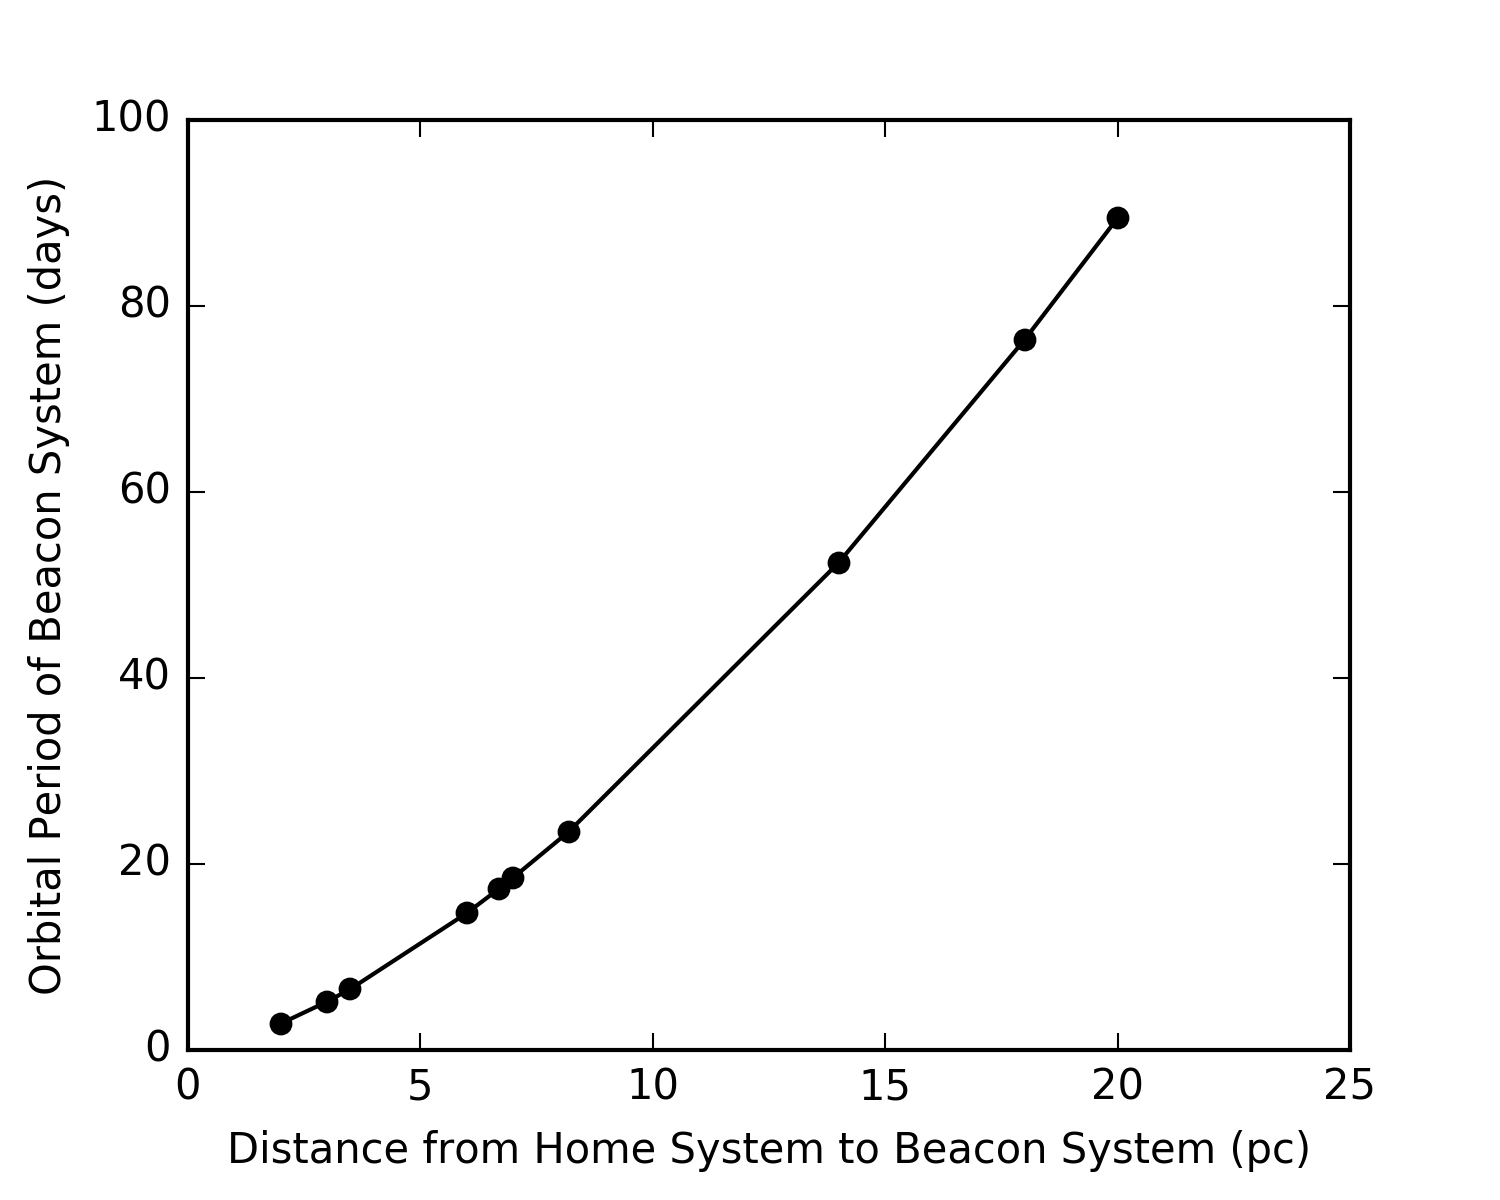
\includegraphics[width=3.5in]{../figures/dist_per.png}
\caption{schematic figure of the signal to detect in 1 dimension}
\label{fig:1d}
\end{figure}


\begin{figure}[]
\centering
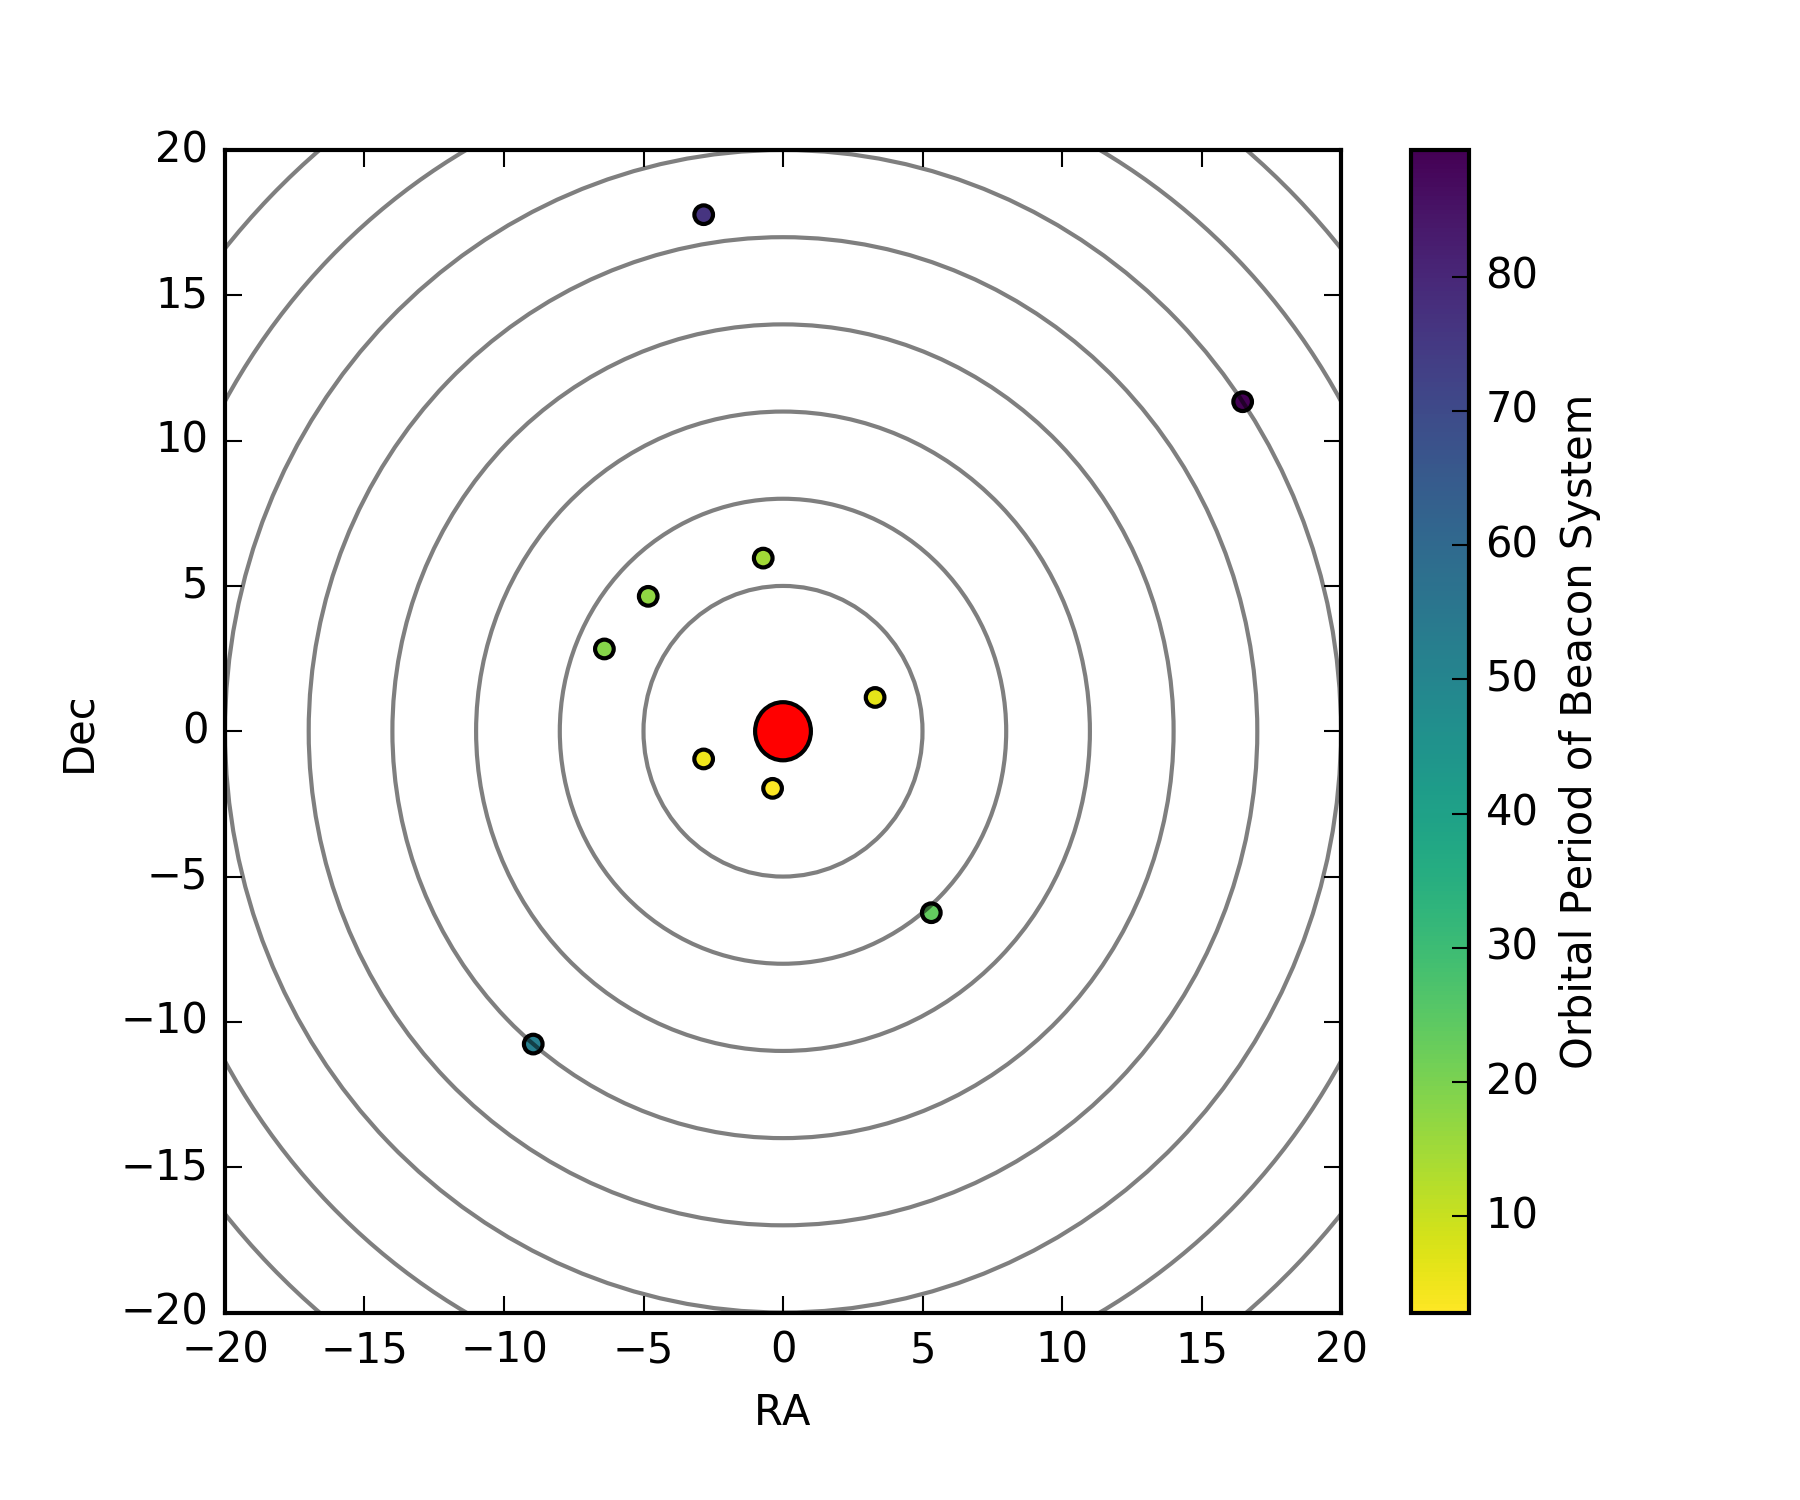
\includegraphics[width=3.5in]{../figures/sky_per.png}
\caption{schematic figure of the signal to detect in 2 dimensions. ra,dec in arbitrary units. red circle in middle is the home system}
\label{fig:2d}
\end{figure}


%%%%%%%%%%%%%%%%%%%%%%%%%%%%%%
\section{Predictions for Upcoming Surveys}
TESS would be great for this in terms of spatial-temporal coverage. 

LSST very good for finding SETI signals of this geometric style, but not ideal for events requiring such dedicating monitoring


%%%%%%%%%%%%%%%%%%%%%%%%%%%%%%
\section{Summary}



%%%%%%%%%%%%%%%%%
\acknowledgments
JRAD is supported by an NSF Astronomy and Astrophysics Postdoctoral Fellowship under award AST-1501418.

\bibliography{/Users/james/research/references}

\end{document}